\documentclass{article}
\usepackage{amsmath}
\usepackage{amsfonts}
\usepackage{amssymb}
\usepackage{mathrsfs}
\usepackage{dsfont}
\usepackage{cancel}

\usepackage{graphicx}


\setlength\parindent{0pt}

\author{Pranav Tikkawar}
\title{PDEs: Homework 2}

\begin{document}
\maketitle

\section*{1.4 Problem 4}
A rod occupying the interval $0 \leq x \leq l$ is subject to the heat source
$f(x) = 0$ for $0 < x < l/2$ , and $f(x) = H$ for $l/2 < x < l$ where $H > 0$. The rod has physical constants $c = \rho = k = 1$, and its ends are kept at zero temperature.
\subsection*{a} 
Find the steady-state temperature of the rod.\\
\textbf{Solution:} \\
$u(0, t) = u(l, t) = 0, \lim_{t \rightarrow \infty} u_t = 0$ and $u(l/2, t)$ is equal on both sides with $u(l/2,t)_x$ are also equal on both sides\\
The steady-state temperature $u(x)$ satisfies the equation
$$ u_{xx} + f(x) = 0 $$
We can then integrate this to get:
\begin{align*}
u_{xx} &= -f(x) \\
u_{x} &= -\int f(x) dx \\
u_{x} &= \begin{cases}
0 + C_1(t) & \text{for } 0 < x < l/2 \\
-Hx + C_2(t) & \text{for } l/2 < x < l
\end{cases}\\
u &= -\begin{cases}
C_1(t)x + C_3(t) & \text{for } 0 < x < l/2 \\
-\frac{H}{2}x^2 + C_2(t)x + C_4(t) & \text{for } l/2 < x < l
\end{cases}
\end{align*}

Now we can apply the boundary conditions.\\

At $x = 0$:
$$u(0,t) = C_3(t) = 0$$
At $x = l$:
$$u(l,t) = -\frac{H}{2}l^2 + C_2(t)l + C_4(t) = 0$$
At $x = l/2$:
$$u(l/2,t) = -\frac{H}{2}\left(\frac{l}{2}\right)^2 + C_2(t)\left(\frac{l}{2}\right) + C_4(t) = C_1(t)\frac{l}{2} + C_3(t)$$
And the partial derivative of x at $x = l/2$:
$$u_x(l/2,t) = -H\left(\frac{l}{2}\right) + C_2(t) = C_1(t)$$

Solving the system of equations we get:
$$T(x) = \begin{cases}
\frac{Hl}{8}x & \text{for } 0 < x < l/2 \\
-\frac{H}{8}(l-4x)(1-x) & \text{for } l/2 < x < l
\end{cases}$$

\subsection*{b} 
Which point is the hottest, and what is the temperature there?
\textbf{Answer:}\\
We can determine the hottest place by taking the derivative of the temperature function and setting it to 0.\\
We can notice that for $0 < x < l/2$ the temperature is linearly increating thus the ottest temperature at that interval will be at $x = l/2$ with a temp of $\frac{Hl^2}{16}$
For $l/2 < x < l$ the temperature derivative is 
$$ T'(x) = H(\frac{5l}{8} - x)$$
For $x = \frac{5l}{8}$ the derivative is 0 and thus the temperature is at a maximum on that interval.\\
Evaluating the temperature at that point we get:
$$ T(\frac{5l}{8}) = \frac{9Hl^2}{128}$$  Since the temp at $x = \frac{5l}{8}$ is greater than the temp at $x = l/2$ the hottest point is at $x = 5l/8$ with a temperature of $\frac{9Hl^2}{128}$




\section*{1.4 Problem 6 }
Two homogeneous rods have the same cross section, specific heat c, and
density $\rho$ but different heat conductivities $\kappa_1$ and $\kappa_2$ and lengths $L_1$ and $L_2$. Let $k_j = \kappa_j/c\rho$ be their diffusion constants. They are welded together
so that the temperature $u$ and the heat flux $\kappa u_x$ at the weld are continuous.
The left-hand rod has its left end maintained at temperature zero. The
right-hand rod has its right end maintained at temperature T degrees.\\
\subsection*{a} Find the equilibrium temperature distribution in the composite rod.
\textbf{Solution:}\\
We can solve this problem by using the heat equation and applying the boundary conditions.\\
The heat equation is given by:
$$ c \rho u_t = \nabla \cdot (\kappa \nabla u)$$
We can notice that since the rod has two seperate conductivities, the heat equation will be different for the two rods.\\
we can Consider the cases
$$\begin{cases}
    c \rho u_{t} = \kappa_1 u_{xx} & \text{for } 0 < x < L_1\\
    c \rho u_{t} = \kappa_2 u_{xx} & \text{for } L_1 < x < L_1 + L_2
\end{cases}$$
Since we want the equilibrium temperature we want the derivative of the temperature to be 0 as it approaches infinity.\\
We also can not that it will not be a function of time and thus we can solve the equation dividing both sizes by the respective $\kappa$ by setting the right hand side to 0.\\
Thus we get the equations:
$$\begin{cases}
    u_{xx} = 0 & \text{for } 0 < x < L_1\\
    u_{xx} = 0 & \text{for } L_1 < x < L_1 + L_2
\end{cases}$$
We can solve these equations by integrating twice to get:
$$\begin{cases}
    u = C_1x + C_2 & \text{for } 0 < x < L_1\\
    u = C_3x + C_4 & \text{for } L_1 < x < L_1 + L_2
\end{cases}$$
The boundary conitions are that $u(0,t) = 0$ and $u(L_1 + L_2, t) = T$ and that the heat flux is continuous at the weld.\\
And at equilibrium $u(0) = 0$ and $u(L_1 + L_2) = T$\\
We also know that the heat flux is continuous at the weld and thus we can say that $\kappa_1 u_x(L_1) = \kappa_2 u_x(L_1)$\\
Thus we can solve the system of equations to get the equilibrium temperature distribution.\\
\begin{align*}
    u(0) = 0 & \implies C_2 = 0\\
    u(L_1 + L_2) = T & \implies C_3(L_1 + L_2) + C_4 = T\\
    \kappa_1 u(L_1) = \kappa_2 u(L_1) & \implies C_1L_1 + C_2 = C_3L_1 + C_4\\
    \kappa_1 u_x(L_1) = \kappa_2 u_x(L_1) & \implies \kappa_1C_1 = \kappa_2C_3
\end{align*}
Solving the system of equations we get:
$$ u(x) = \begin{cases}
    \frac{\kappa_2T}{\kappa_2L_1 + \kappa_1L_2}x & \text{for } 0 < x < L_1\\
    T - \frac{\kappa_1T}{\kappa_2L_1 + \kappa_1L_2}(L_1+L_2-x) & \text{for } L_1 < x < L_1 + L_2
\end{cases}$$


\subsection*{b} Sketch it as a function of x in case $k_1 = 2, k_2 = 1, L_1 = 3, L_2 = 2, \text{ and } T = 10$. (This exercise requires a lot of elementary algebra, but
it's worth it.)
\textbf{Solution:}\\
Setting these values into the equation we get:
$$ u(x) = \begin{cases}
    \frac{10}{7}x & \text{for } 0 < x < 3\\
    \frac{10}{7}(2x-3) & \text{for } 3 < x < 5
\end{cases}$$

\begin{center}
    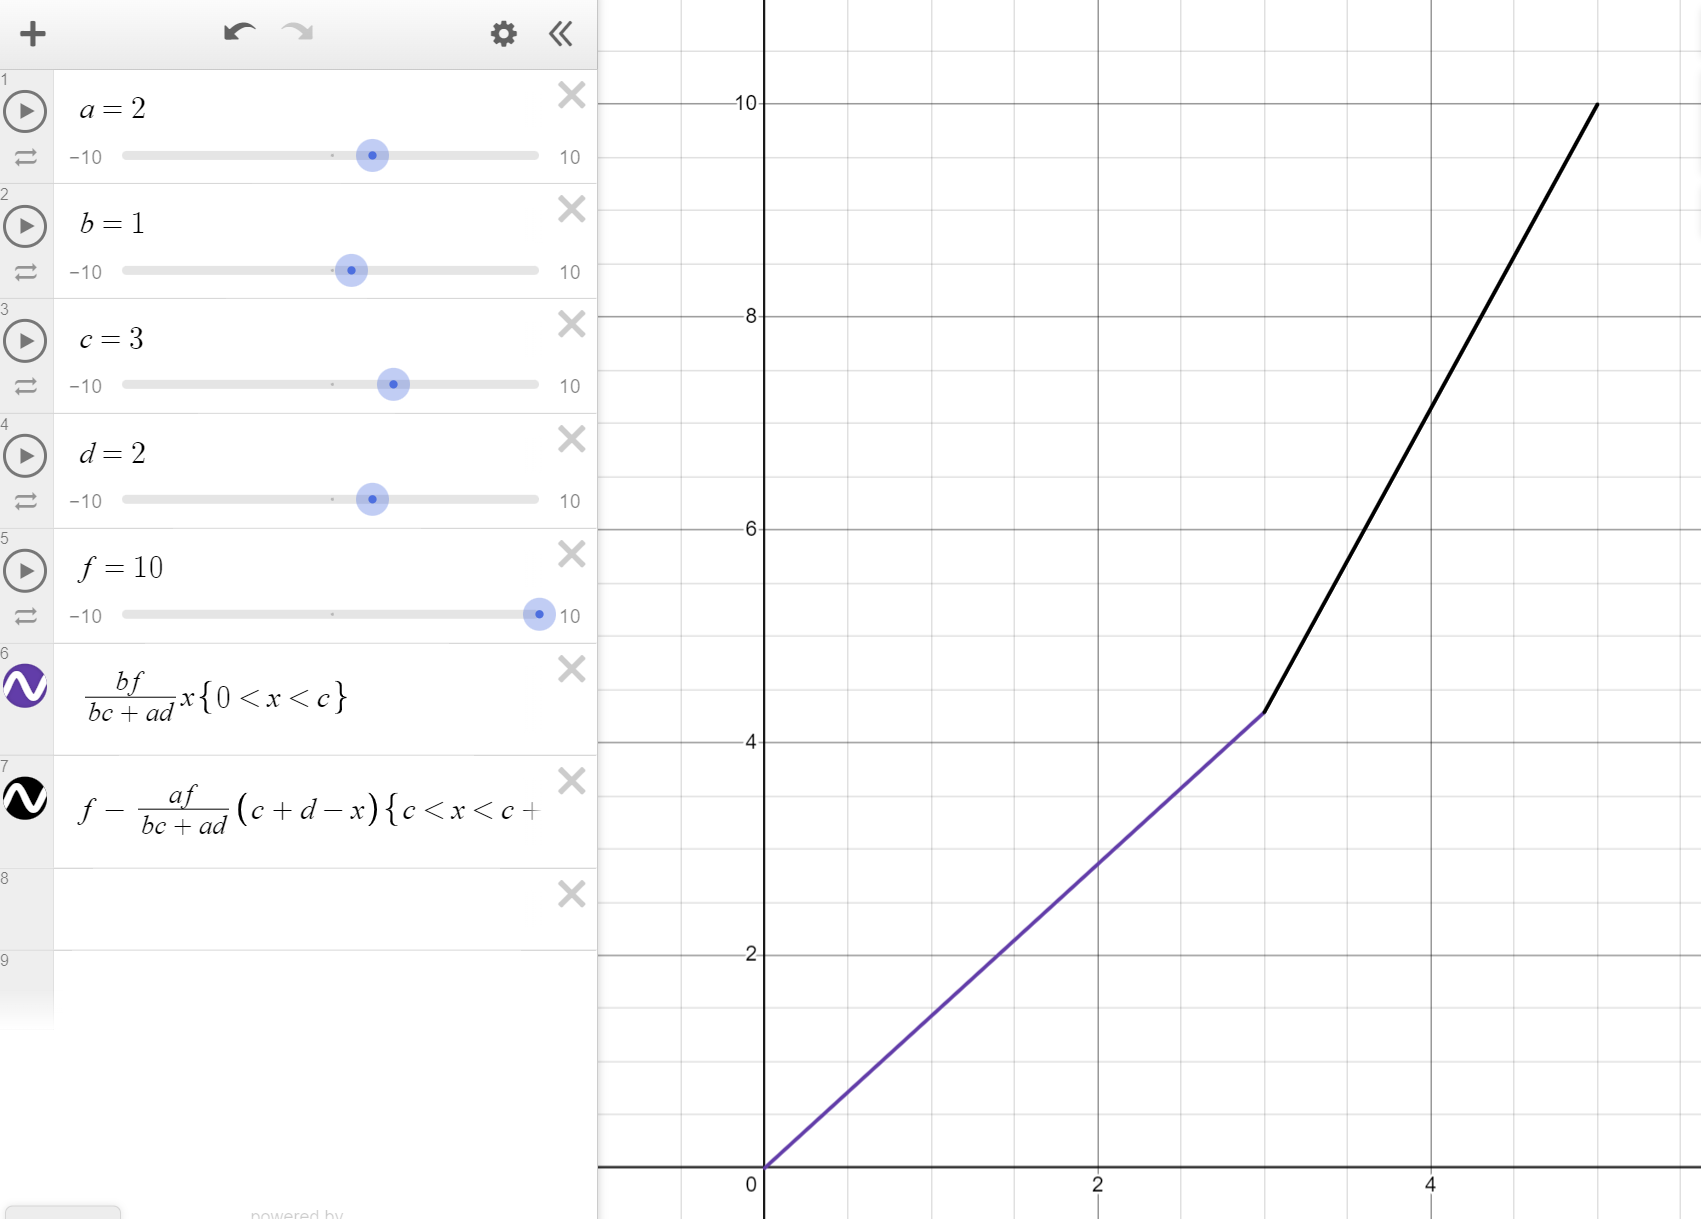
\includegraphics[scale=0.25]{IMGs/HW2plot.png}
\end{center}


\section*{1.5 Problem 2 }
Consider the problem 
$$ u''(x) + u'(x) = f(x)$$
$$ u'(0) = u(0) = \frac{1}{2}[u'(l) + u(l)]$$
With $f(x)$ a given function.\\
\subsection*{a} Is the solution unique? Explain.\\
We can prove uniqueness by showing there are 2 solutions and then showing that they are equal.\\
We can let $u_1$ and $u_2$ be solutions to the problem.\\
Then we can let $w = u_1 - u_2$ and show that $w = 0$.\\
Since $u_1, u_2$ are solutions to the problem, we can substitute them into the equation to get:
\begin{align*}
    u_1'' + u_1' &= f(x)\\
    u_2'' + u_2' &= f(x)
\end{align*}
Subtracting the two equations we get:
$$ w'' + w' = 0$$
This is a second order linear equation and we can solve it by integrating factor of $e^{-x}.$\\
Thus we get the solution $w = C_1e^{-x}$\\
Clearly $C_1e^{-x} \neq 0$ for all $x$ so $w \neq 0$ and thus the solution is unique.\\

\subsection*{b} Does a solution necessarily exist or is there a condition that $f(x)$ must satisfy for a solution to exist?\\
% We can show existance, through boundary condition, show that f must have specific conditions for a solution to exist.\\
% Integrate both sides and pplly boundary conditions to get the conditions on f.\\
% Thus f is not nessarily arbitrary, it must satisfy the conditions.\\
We can show exitance through the boundary conditions.\\
We can do this by integrating both sides of the equation and applying the boundary conditions.\\
\begin{align*}
    \int_0^l u''(x) + u'(x) dx &= \int_0^l f(x) dx\\
    [u'(l) + u(l)] - [u'(0) + u(0)] &= \int_0^l f(x) dx\\
    0 &= \int_0^l f(x) dx
\end{align*}
Thus we need to have that $f(x)$ is such that $\int_0^l f(x) dx = 0$ for a solution to exist.\\



\section*{1.5 Problem 6}
Solve the equation 
$$ u_x + 2xy^2 u_y = 0$$
\textbf{Solution: }\\
We solve this by noticing the directional derivative in the direction of the vector $(1, 2xy^2)$ is 0. This means that the solution is constant along the lines $y^2 = x^2 + C$ for some constant $C$.\\
Thus we can also say that 
$$ \frac{dy}{dx} = \frac{2xy^2}{1} = 2xy^2$$
This is a separable differential equation and we can solve it by separating the variables and integrating.\\
\begin{align*}
    \frac{dy}{dx} &= 2xy^2\\
    \int y^{-2} dy &= \int 2x dx\\
    -y^{-1} &= x^2 + C\\
    y &= \frac{-1}{x^2 + C}
\end{align*}
Thus we can say our solution will be in the form of $u(x,y) = u(x, \frac{-1}{x^2 + C})$.\\
% solve for c and then plug in to get the solution
For any x, the characteristic curve only depends on C and not x
We can see this if we take $x =0$ as 
$$ u(0, \frac{1}{C}) = f(C)$$ 
For some arbitrary function $f(C)$\\
Since we can see that $C = x^2 + y^{-1}$ we can substitute this into the equation to get the solution.\\
Thus $u(x,y) = f(x^2 + y^{-1})$ for some arbitrary function $f$.


\section*{1.6 Problem 4}
What is the type of the equation:
$$ u_{xx} - 4u_{xy} + 4u_{yy} = 0$$
Show that by direct substition that $u(x,y) = f(y+2x) + xg(y+2x)$ is a solution for arbitrary functions $f$ and $g$. \\
\textbf{Solution:}\\
This is a parabolic equation due to $b^2 - 4ac = 16 - 16 = 0 $ \\
To prove that $u(x,y) = f(y+2x) + xg(y+2x)$ is a solution we can substitute it into the equation and show that it satisfies the equation.\\ 
\begin{align*}
    u_{xx} &= 4f''(y+2x) + 2g'(y+2x) + 2g'(y+2x) + 4xg''(y+2x)\\
    u_{xy} &= 2f''(y+2x) + g'(y+2x) + 2xg''(y+2x)\\
    u_{yy} &= f''(y+2x) + xg''(y+2x)\\
    u_{xx} - 4u_{xy} + 4u_{yy} &= 4f''(y+2x) + 2g'(y+2x) + 2g'(y+2x) + 4xg''(y+2x)\\ &- 8f''(y+2x) - 4g'(y+2x) - 8xg''(y+2x) + 4f''(y+2x) + 4xg''(y+2x)\\
    &= 0
\end{align*}


\section*{1.6 Problem 6 }
Consider the equation
$$ 3u_y + u_{xy} = 0$$
\subsection*{a}
What is its type?\\
Hyperbolic\\
\textbf{Solution:}\\
This is a hyperbolic equation due to $b^2 - 4ac = 1 - 0 = 1$\\

\subsection*{b}
Find the general solution. Hint ($v = u_y$)\\
\textbf{Solution:}\\
We can preform a subsection of $v = u_y$ to get a first order linear equation.\\
$$ 3v + v_x = 0$$
This is a first order linear equation and we can solve it by separating the variables and integrating.\\
Thus results in the solution $v = {C_1(y)}e^{-3x}$\\
Where $C_1(y)$ is an arbitrary function of $y$.\\
Replacing $v$ with $u_y$ we get:
$$ u_y = C_1(y)e^{-3x}$$
We can now solve this by separating the variables and integrating.\\
\begin{align*}
    u_y = C_1(y)e^{-3x}
    \int du = e^{-3x}\int C_1(y) dy\\
    u = e^{-3x}C_2(y) + C_3(x)
\end{align*}
Where $C_2(y) = \int C_1(y) dy $ which is arbitrary and $C_3(x)$ is an arbitrary function of $x$.\\ 


\subsection*{c}
With auxiliary conditions $u(x,0) = e^{-3x}$ and $u_y(x,0) = 0$, does a solution exist? Is it unique?\\
We can determine if a solution exists and is unique by applying the boundary conditions to the general solution.\\
\begin{align*}
    u(x,0) = e^{-3x} &= e^{-3x}C_2(0) + C_3(x)\\
    u_y(x,0) = 0 &= C_1(0)e^{-3x}\\
\end{align*}
From the second equation we can see that $C_1(0) = 0$ and thus $u_y = 0$ for all $x$ and $y$.\\
But this not nessarily mean that the solution is unique.\\
We can find two functions of $C_2(y)$ and $C_3(x)$ that satisfy the first equation.\\
For example we can let $C_2(y) = 1$ and $C_3(x) = 0$ and $C_2(y) = 2$ and $C_3(x) = -e^{-3x}$.\\
Thus the solution is not unique.\\


\end{document}